\documentclass[tikz, border=0.2cm]{standalone}
\usetikzlibrary{positioning}

\begin{document}
\tikzset{
	every node/.style={draw=black, circle, minimum size=3em, node 
	distance=4em}
}

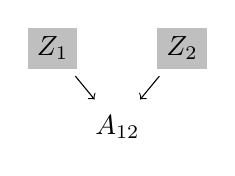
\begin{tikzpicture}[shorten >=3pt, shorten <=3pt]
% Nodes
\node[fill=gray!50!white] (z1) {\(Z_1\)};
\node[fill=gray!50!white, right=of z1] (z2) {\(Z_2\)};
\path (z1) -- (z2) coordinate[midway] (aux);
\node [below of=aux] (a) {\(A_{12}\)};

% Arrows
\draw[->] (z1) -- (a);
\draw[->] (z2) -- (a);
\end{tikzpicture}

\end{document}
